%%==================================================
%% chapter01.tex for BIT Master Thesis
%% modified by yang yating
%% version: 0.1
%% last update: Dec 25th, 2016
%%==================================================
\chapter{绪论}
\label{chap:intro}
\section{研究背景及意义}

科学技术总是能让我们生活变得更加美好,它的发展经常在我们的意料之外,特别是机器人这个行业,在过去几十年里发展迅速。银行大厅里可爱的机器人助手、现代化餐厅的送餐机器人、室内清扫机器人、儿童手中的无人机玩具等,这些移动机器人都是现代机器人技术发展的结晶。世界上很多研究机构,例如波士顿公司和MTI等,正在研究仿生机器人,并且取得了显著的成果。随着人工智能和5G技术的快速发展,机器人行业的一个分支——无人驾驶技术,正成为国际上一个重要的研究方向和热点。所有这些机器人都有一个共同点——自主性,拥有在不熟悉的环境中移动而不依赖外部信息和控制的能力。自主定位与导航技术为实现这一共性提供了基础。

SLAM是Simultaneous Localization and Mapping的缩写,译为“同时定位与地图构建”\upcite{Zhaopeng2015}。它是指携带有特定传感器的移动载体,在未知的陌生环境下,边运动边感知周围环境,并构建地图,同时估计出本体在地图中的位置\upcite{davison2007monoslam}。大多数机器人实现自主定位用的都是SLAM技术。SLAM可以使用激光传感器,称为激光SLAM。也可以使用视觉传感器,称为视觉SLAM,简称VSLAM(Visual SLAM)。早期研究者大都以激光SLAM研究为主,现今,随着计算机硬件和软件的极速发展,视觉SLAM凭借着信息量大、体积小、重量轻、适用范围广和成本低等优点受到广泛关注,逐渐成为研究者心中的热门研究领域。

然而视觉SLAM本身也存在着诸多问题,比如当相机运动过快时图像出现模糊或者前后两帧没有重叠区域导致特征匹配失败,无法应对特征缺失和大面积重复纹理场景,光照变化幅度大时跟踪容易失败等等。惯性测量单元(Inertial Measurement Unit,IMU)输出频率高,在短时间内对快速运动估计较为准确。大多数IMU读数漂移严重,而相机的漂移较小。相机属于外感受型传感器,当图像变化时我们无法知道是相机在运动还是周围环境发生了变化,所以纯视觉SLAM常常难以应对动态场景。而IMU属于内感受型器,能够感受到自身的6-DoF(六自由度)运动信息。因此相机和IMU被认为是一对具有互补性的传感器。在大多数情况下,最好的状态估计就是同时有效利用内感受型和外感受型传感器的观测值\upcite{barfoot2017state}。因此视觉/惯性融合成为目前学术界的研究热点。

%  1.2
\section{国内外研究现状}
%\label{sec:***} 可标注label
SLAM技术已经有30多年的历史了,伴随着计算机硬件的巨大改进,研究热点从激光转移到视觉。有部分研究者提出了划时代的理论算法,为SLAM的发展奠定了理论基础。还有部分研究者实际研究并编程实现了SLAM的各种算法的完整框架,甚至开源了他们的源代码,为SLAM的发展做出了无私的贡献。正是因为有很多这样孜孜不倦、无私奉献的学者,SLAM技术才能日渐成熟,走向大众。

下面,本文将首先对视觉SLAM的发展历程和有影响力的研究成果经行概述,然后对视觉/惯性融合的发展现状经行详细阐述。

%  1.2.1
\subsection{视觉SLAM研究概述}
%\label{sec:features}

SLAM最早叫做概率SLAM(probabilistic SLAM)。早期大多以激光传感器为主,SLAM中存在一个基本问题——全局一致性。Cheesman\upcite{smith1986representation}和Durrant-Whyte\upcite{durrant1988uncertain}为了描述路标与路标之间的相互关系而建立了一个统计学框架,该框架主要用来解决几何上的不确定性。他们证明了估计的路标位置之间具有强关联性,并且这种关联性会随着观测的时间增加而增加。

%6
Ayache和Faugeras最先从事视觉SLAM的研究。Smith等人提出移动机器人在陌生环境中获取的路标时,因为这些路标具有相同的估计误差,所以路标的估计值也是相关的\upcite{smith1990estimating}。这样就加大了难度。因为状态向量中将包含机器人的位姿和每一个路标点的观测值,而且每观测一次都要实时更新,这导致状态向量的维数非常大,进而带来巨大的计算量。SLAM中的地图有一个收敛的性质,因为Smith等人将其忽略,并假设地图的估计误差是发散的,因此学者们只能视路标点之间没有相关性或者相关性很小。这是因为这个原因,当时的SLAM大都是将定位和建图问题分开处理的。

%[7][8]

1995年文章International Symposium on Robotics提出了收敛性和同时定位建图的概念\upcite{durrant1996localization},此时研究者们才将定位与地图构建问题结合在一起,突破了新的理论。之后SLAM的研究集中在计算速度的提升以及多源信息融合上。在ISRR99上,Thrun首次提出将基于卡尔曼滤波(Kalman filter)的SLAM与概率定位建图相结合\upcite{thrun1998probabilistic}。

进入二十一世纪后,因为计算机硬件性能的提升,研究热潮逐渐转向以相机为传感器的视觉SLAM,并出现了很多可以实现的理论框架,甚至有一些理论框架已经落地市场化。

%[9][10][11]

A. J. Davison可以说是视觉SLAM领域中的领头人,他在单目视觉SLAM中做了奠基性的工作\upcite{davison2007monoslam}\upcite{Davison03real-timesimultaneous},极大的推动了视觉SLAM的发展。他在2007年的一篇文章中提出了MonoSLAM\upcite{davison2007monoslam},该系统有一个重大突破——可以实时运行。MonoSLAM仅仅依靠单目相机,检测每一帧图像中的Shi-Tomasi角点,该角点是很稀疏的角点,然后在投影椭圆中实施特征匹配。经典的扩展卡尔曼滤波器(EKF)被用于SLAM后端,路标点的位置被建模为高斯分布,位姿及其关联的路标点构成状态向量,并实时更新其均值和协方差。

%[11][12]

Klein等人在2007年提出并开源了PTAM(Parallel Tracking and Mapping)\upcite{klein2007parallel},并在两年后将PTAM算法移植到智能手机上\upcite{klein2009parallel}。PTAM首次提出并编程实现了前端特征跟踪和后端建图的并行化,将前端和后端分开来并行计算,这是一个值得称赞的突破。时至今日,这种思想仍在继续使用,效果极好。此外,PTAM还创新地使用了关键帧机制,这一重大创新使得处理器不必处理每一帧图像,而是处理几个关键的图像,大大减少了计算量。而且,对比MonoSLAM,PTAM在后端不使用卡尔曼滤波器。取而代之的是非线性优化,这在历史上是第一次的。这一开创性突破直接导致了在PTAM之后,研究者开始以非线性优化为主来设计后端算法。并采取关键帧机制和多线程并行化思想。PTAM对视觉SLAM研究提出了很多创新的算法和重大革新,对视觉SLAM的发展做出了巨大的贡献。

%[13][14][15]

Raul Mur-Artal等人在2015年提出了ORB-SLAM系统\upcite{mur2015orb}。如果说MonoSLAM和PTAM是在时间上距离我们较为久远的方案,那么ORB-SLAM则是距离我们很近的全新的方案。ORB-SLAM是自2015年以来所有纯视觉SLAM算法中最为优秀的算法之一。ORB-SLAM提出了自己独特的创新和改进,抛弃了传统的SIFT(Scale Invariant Feature transform)\upcite{lowe2004distinctive}和SURF(Speeded Up Robust Features)\upcite{bay2008speeded}特征,采用自己独特的ORB特征进行特征提取。相比于SIFT和SURF,ORB特征计算快,可以在处理器上实现实时计算。与Harris角点相比,ORB特征点比Harris角点多了一个尺度不变特性以及描述子,可以快速的进行特征匹配、回环检测或者重定位。因此,ORB特征是一种折衷了计算速度和计算精度的优秀特征方案。在回环检测中ORB-SLAM使用了ORB字典,大大减少了系统的累计误差,同时在特征丢失之后也能快速找回,大大提高了整个系统的鲁棒性。最后,该系统创新地使用了三线程并行方案。使得前端、后端和回环各自有条不紊的工作。ORB-SLAM是主流特征点法的巅峰之作,极大的推动了视觉SLAM技术的发展。

MonoSLAM、PTAM和ORB-SLAM的运行效果如图\ref{fig1_1}所示。

\begin{figure}[h]\setlength{\belowcaptionskip}{-12pt}
	\centering
	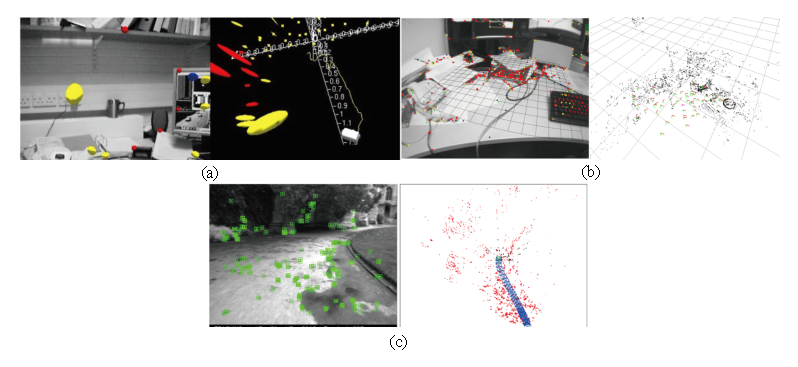
\includegraphics[width=0.75\textwidth]{figures/chapter1/fig1_1}
	\caption{(a) MonoSLAM;(b) PTAM;(c) ORB-SLAM.}\label{fig1_1}
\end{figure}

以上所介绍的视觉SLAM系统都是基于特征点的方案,称作特征点法或者间接法。特征点是人为从图像中提取和设计的特殊的角点,一般包括关键点和描述子。在视觉SLAM的前端跟踪中用来代替整张图片的纹理,在后端中将其视为路标点进行迭代优化。特征点的存在使得相机在运动的过程中,SLAM系统前端跟踪也能取得良好的效果。万事有利必有弊,虽然特征点法应用广泛,鲁棒性高,但是特征点法仍然有缺点:提取关键点需要花费很长时间;提取特征点意味着主动丢掉了图像中的其他信息;在一些单色无纹理区域,往往很难提取特征点,在重复纹理区域,特征点普遍跟踪混乱,无法使用。

除了特征点法,近几年来研究者们也在研究一种基于像素的直接法。直接法与光流法非常相似,其灰度不变性的假设是应用的前提。该方法不需要提取图像特征点,而是通过最小化亮度误差直接估计像素深度,从而计算像素3D空间位置和相机的运动。因此,直接法相比于特征点法在计算速度上有很大提升,并且能适应特征缺失和图像模糊的场景。同时,直接法仅用CPU就能构建稀疏或者半稠密地图,这是特征法做不到的。


%[16][17]
2014年,TUM计算机视觉组的J. Engel 等人提出LSD-SLAM\upcite{engel2014lsd}\upcite{engel2013semi},LSD-SLAM采用直接法,可以构建半密集三维地图。这是单目直接法在视觉SLAM中的典型应用。与以往的方案不同,LSD-SLAM仅使用CPU就可以完成半密集地图的三维重建。LSD-SLAM有很多自己的创新之处,例如,LSD-SLAM既不是利用像素,也不是利用块匹配去跟踪图相机,而是在极线上等间距的取五个点,计算其SSD(Sum of Squared Distance);LSD-SLAM没有复杂的初始化过程,而是对深度随机赋值,然后在将计算出来的深度归一化,得到全局一致的尺度;使用光度不确定性项来计算深度协方差;使用李群和李代数 来对关键帧进行约束,在后端优化中考虑不同的尺度,进而减小大范围场景中的尺度漂移现象。

%[18]
Forster 等人在2014年提出SVO(Semi-direct Visual Odoemtry)\upcite{forster2014svo}。SVO采用稀疏直接法,也称作“半直接法”。之所以成为“半直接法”,是因为SVO同时使用了特征点法和直接法,在前端提取角点,然后利用角点周围的信息通过直接法估计出相机的运动以及自身的位置。该方案对比于其他方案,显著的优势是速度极快,它甚至可以在低端处理器上实现实时计算,这使得SVO可以应用到无人机、智能手机、VR等设备上。另外,SVO在理论上也有一个重大的创新,提出了深度滤波器的概念。在估计角点的位置时,逆深度被用来设计参数,使之能够更好的计算特征点位置。

LSD-SLAM和SVO的运行效果如图\ref{fig1_2}所示。

\begin{figure}[h]\setlength{\belowcaptionskip}{-12pt}
	\centering
	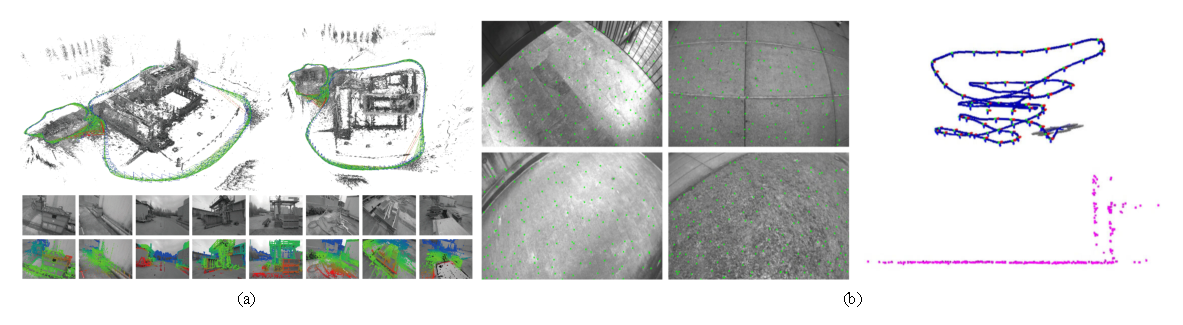
\includegraphics[width=0.75\textwidth]{figures/chapter1/fig1_2}
	\caption{(a) LSD-SLAM;(b) SVO.}\label{fig1_2}
\end{figure}

%[19][20][21][22][23][24][25][26][27]
国内SLAM的研究因为起步较晚,所以一直落后于国外,但是,近几年来随着自动驾驶行业的发展,SLAM研究越来越受到重视。很多高校都在开展SLAM相关的课题研究,也出现了一些详细解读SLAM技术的文章\upcite{权美香2016视觉}\upcite{刘浩敏2016基于单目视觉的同时定位与地图构建方法综述}\upcite{何俊学2010基于视觉的同时定位与地图构建方法综述}。上海交通大学的邹丹平等人提出了基于线特征的StructSLAM\upcite{zhou2015structslam}以及基于多目相机的Co-SLAM\upcite{zou2013coslam}。浙江大学计算机学院的章国锋等人于2013年提出了RDSLAM\upcite{tan2013robust},RDSLAM的创新之处是将传统的随机采样一致性(RANSAC)\upcite{fischler1981random}算法改为一种基于时间序列和先验信息的自适应RANSAC算法,该算法弥补了之前算法在动态场景下表现欠佳的缺点。2016年,他们又提出了改进版的基于移动设备的RKSLAM\upcite{liu2016robust},可以实时运行。2017年,他们提出基于RGB-D相机的RKD-SLAM系统\upcite{liu2017robustRGB},RKD-SLAM能够构建稠密地图。

%1.2.2
\subsection{视觉/惯性融合研究概述}
%\label{sec:requirements}

尽管仅用相机就能完成定位和建图任务的视觉SLAM。然而,纯视觉SLAM往往因为各种各样的问题导致其应用场景有限,鲁棒性低。广大学者和工程师往往希望算法能够得到实际的应用,而不是局限于在个人PC上跑demo。在这种应用需求的背景下,视觉与惯性融合的定位方案逐渐成为学术界的研究热点。

%[28]
目前的VIO算法可以分为松耦合和紧耦合\upcite{martinelli2014closed}。松耦合将相机和IMU分开处理,各自单独估计,然后将二者估计出的结果进行融合。紧耦合是指将IMU和相机的状态量融合在一起,组成一个整体的状态方程。然后对状态方程进行求解。类比于纯视觉SLAM,VIO也可以分为基于滤波和基于优化两大类。下面将基于这几种分类对VIO的研究现状进行分析。

%[29][30][31]
宾夕法尼亚大学Kumar实验室的Mourikis等人于2007年提出基于滤波的紧耦合VIO方案——MSCKF(Multi-State Constraint KF)\upcite{mourikis2007multi},并于2015年提出了改进的MSCKF\upcite{li2013high}。传统的EKF-SLAM(Extended kalman filtering SLAM)\upcite{bloesch2015robust}系统会将图像的特征信息加入到状态向量和协方差矩阵里,如果在初始化特征点深度和协方差矩阵的时候有误差,那么很容易造成全局轨迹不一致的情况。而MSCKF始终保持一个先进先出的滑动窗口序列,在滑窗内建立EKF的预测和更新。

%[32]
苏黎世联邦理工学院自动控制系统实验室的Stephen Weiss等人于2013年提出基于滤波的松耦合VIO方案——SSF和MSF\upcite{lynen2013robust}。松耦合系统没有紧耦合系统那么繁杂,而且MSF可以用来融合除相机和IMU之外的其他多种传感器。松耦合还有另一个优点:当一个传感器不能工作时,系统任然能够依靠其他传感器正常运行。紧耦合系统则是所有传感器相互依赖,缺一不可。

%[33][34]
2014年,苏黎世联邦理工学院的Stefan Leutenegger等人提出基于优化的紧耦合VIO方案——OKVIS\upcite{Leutenegger_keyframe-basedvisual-inertial}。OKVIS在一个滑窗内优化关键帧,带权重的视觉重投影误差和带权重的IMU误差组成残差项。前端提取尺度不变的Harris特征点,并计算BRISK描述子\upcite{leutenegger2011brisk},后端使用非线性优化的方式进行状态估计。另外OKVIS同时支持单目和双目两种类型的相机,Leutenegger的实验表明在双目情况下有更好的效果。

%[35][31]
2015年,苏黎世联邦理工学院的Michael Bloesch等人提出了基于滤波的紧耦合VIO方案——ROVIO\upcite{bloesch2015robust}。ROVIO利用EKF进行状态估计,而且有许多创新的地方。首先,ROVIO在提取角点时采用的是FAST角点\upcite{smith2002fast},使用矢量坐标点方向,用标量表示坐标点大小;其次,图像块用于描述所有的角点,视频流用于多级表达;最后使用惯导计算出的位姿估计视觉重投影的光度误差,并将其用于后端优化。ROVIO仅仅支持单目相机。

%[36]
2017年,香港科技大学的沈绍杰等人提出基于优化的紧耦合VIO方案——VINS-Mono\upcite{qin2018vins}。VINS-Mono是一个基于滑动窗口的紧耦合非线性优化系统。在初始化阶段,通过松耦合的方式融合相机和IMU,从而获得位置、姿态和尺度的初始值。在后端通过IMU残差、视觉残差和边缘化残差构成目标函数,用非线性优化进行计算状态量。值得注意的是,VINS-Mono还具有回环检测和重定位的功能,并在检测到回环时进行4-DoF全局位姿图优化。VINS-Mono在精度和鲁棒性上都表现优异,是一个极具实用价值的VIO开源方案。

%[37]
基于优化的松耦合方案不多,因为学术界普遍认为其效果没有紧耦合好。2016年,Gabe Sibley等人在其文章中提到了基于优化的松耦合方法\upcite{falquez2016inertial}。简而言之,就是将前端计算出的位姿进行坐标变换,然后放到IMU的优化框架中。

目前,VIO算法已经应用在包括自动驾驶、飞行机器人和VR/AR等领域。视觉/惯性融合方案总结如图1.3。本文将对基于优化的紧耦合VIO方案进行细致的研究,并基于单目相机、IMU和磁力计实际搭建一套高精度、简单易用的视觉/惯性/地磁等多传感器融合定位系统。

\begin{figure}[h]\setlength{\belowcaptionskip}{-12pt}
	\centering
	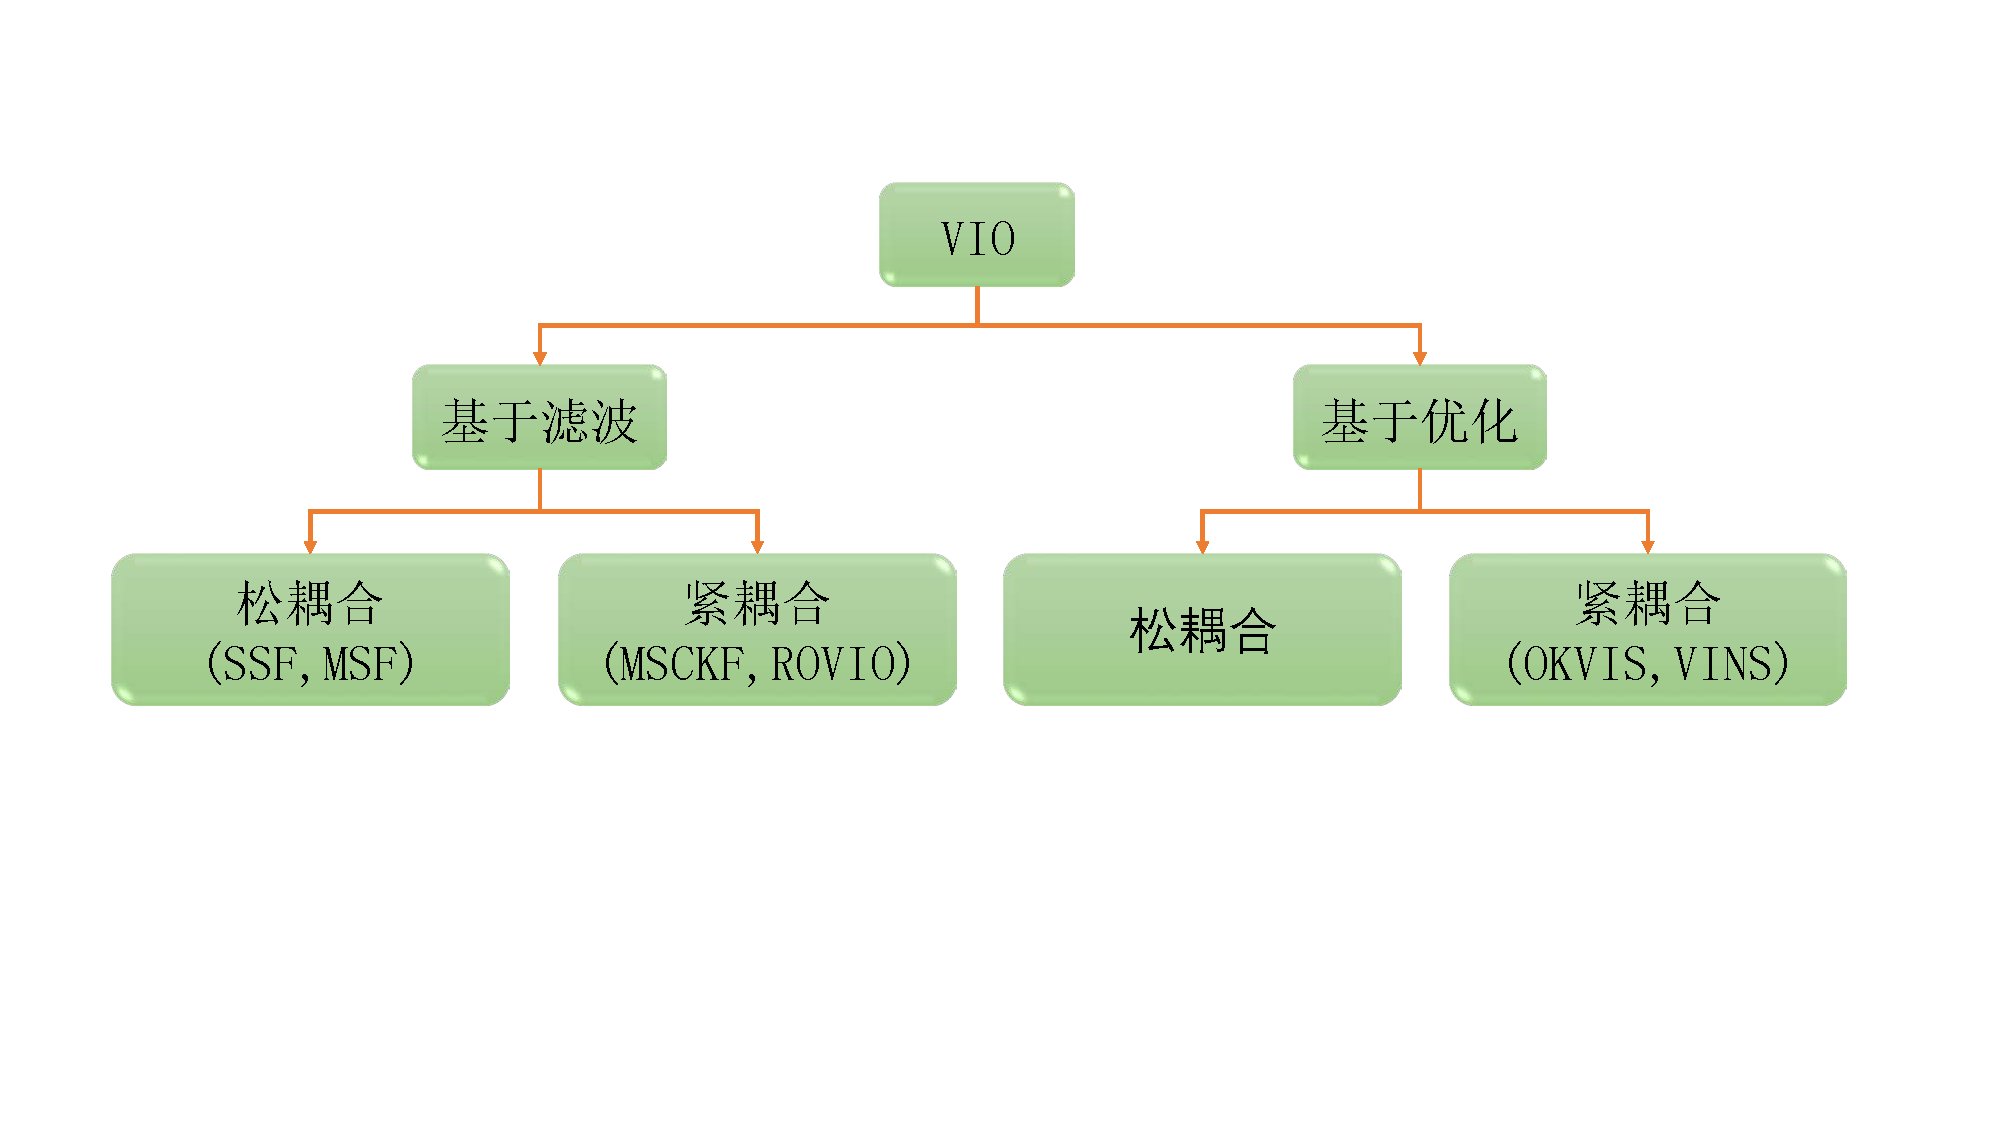
\includegraphics[width=0.75\textwidth]{figures/chapter1/fig1_3}
	\caption{(a) LSD-SLAM;(b) SVO.}\label{fig1_3}
\end{figure}


%  1.3
\section{本文主要工作及结构安排}

本文以视觉/惯性融合为主,磁力计为辅,研究多传感器融合定位算法,并实际搭建一套软硬件结合的多传感器融合定位系统。

本文主要工作如下:

(1)	搜集并研读国内外视觉SLAM和VIO相关的论文,详细阐述了视觉SLAM和VIO的国内外发展现状;

(2)	与市场上普通的消费级视惯套件不同,本文对高精度的工业级传感器进行硬件同步,搭建了一套高精度的多传感器融合定位系统硬件平台;

(3)	研究了视觉SLAM算法、多传感器融合算法,针对自己的硬件系统设计前端、后端及闭环算法,并创新的实现了运动中在线实时初始化和绝对航向初始化;

(4)	在ROS下编程实现所有算法,整个系统拥有良好的可视化功能,可扩展性强;

(5) 进行公开数据集实验和本地实验,分析了系统在不同环境下的定位精度,验证了系统的可行性。

本文各个章节安排如下:

第二章主要研究了系统的硬件平台。首先研究了传感器(相机和IMU)的数学模型及选型;然后研究传感器的标定以及硬件同步原理;最后研究了基于ROS的传感器信息采集方法。

第三章主要研究系统的前端和初始化算法。首先研究视觉信息预处理算法;然后研究IMU预积分原理;最后研究了系统初始化流程,包括纯视觉初始化和视觉/惯性联合初始化。

第四章主要研究系统后端和闭环算法。首先研究了后端非线性优化的方法;然后研究了闭环检测算法;最后研究了重定位和闭环优化算法。

第五章主要是实验。验证算法有效性,并分析定位误差。包括公共数据集实验和本地校园环境实验。

